\documentclass{bioinfo}
\copyrightyear{2015} \pubyear{2015}

\access{Advance Access Publication Date: Day Month Year}
\appnotes{Manuscript Category}
\usepackage{graphicx}

\newcommand{\fixme}[1]{\textcolor{red}{FIXME: #1}}
\usepackage{hyperref}

\begin{document}
\firstpage{1}

\subtitle{Subject Section}

\title[MsQuality: Calculation of standardized quality metrics of mass spectrometry data]{MsQuality – an interoperable open-source package for the calculation of standardized quality metrics of mass spectrometry data}

\author[1,$\ast$]{Thomas Naake}
\author[2]{Johannes Rainer}
\author[1]{Wolfgang Huber}


\author[Naake \textit{et~al}.]{Thomas Naake\,$^{\text{\sfb 1}}$, Johannes Rainer,$^{\text{\sfb 2}}$ and Wolfgang Huber\,$^{\text{\sfb 1}*}$}

\address{}

\address{
$^{\text{\sf 1}}$ Genome Biology Unit, European Molecular Biology Laboratory, Heidelberg, 69117, Germany \\
$^{\text{\sf 2}}$ Institute for Biomedicine (Affiliated to the University of L\"ubeck), Eurac Research, Viale Druso 1, 39100 Bolzano, Italy}


\corresp{$^\ast$corresponding author.}

\history{Received on XXXXX; revised on XXXXX; accepted on XXXXX}
\editor{Associate Editor: XXXXXXX}

\abstract{
\textbf{Motivation:} Multiple factors can impact accuracy and reproducibility
of mass spectrometry data. There is a need to integrate quality
assessment and control into data analytic workflows. \\
\textbf{Results:} The \texttt{MsQuality} package calculates % and assesses 
% various quality metrics for mass spectrometry-derived spectral data at the 
% per-measurement level. It calculates
% ---
% Above seems redundant, no additional information content?
% - what is 'per-measurement level' (what is a 'measurement' -- I think you need to be more specific here, or just drop the phrase
% - why 'around' 40? can you not count them and give the precise number?
%
around 40 low-level quality metrics based on the controlled vocabulary of the mzQC quality
metrics defined by HUPO-PSI.  It helps identify low-quality measurements and track data
quality.  Its use of community-standard quality metrics facilitates comparability of
quality assessment and control (QA/QC) criteria across datasets.\\
%ultimately improving the quality and reproducibility of mass spectrometry 
%data for robust scientific discoveries. \\
\textbf{Availability:} The R package \texttt{MsQuality} is available through 
Bioconductor at https://bioconductor.org/packages/MsQuality.\\
\textbf{Contact:} \href{wolfgang.huber@embl.org}{wolfgang.huber@embl.org}\\
\textbf{Supplementary information:} Supplementary data are available at \textit{Bioinformatics}
online.}

%\keywords{quality control, mass spectrometry, metabolomics, proteomics, R}

\maketitle

Mass spectrometry (MS) is a versatile analytical technique that has been adopted in a
variety of disciplines, including proteomics, metabolomics, and lipidomics. MS enables the
identification and quantification of a wide range of molecules. Obtaining high-quality
data from mass spectrometry experiments can be a challenging task, as numerous factors can
impact the accuracy and reproducibility of the obtained data. To ensure that MS data is
fit for purpose, quality assessment and quality control (QA/QC) need to be performed close
% see e.g. Wikipedia for the difference between QA and QC in case it's not clear
to data production \citep{Koecher2011}. Use of standardized quality metrics described by a
controlled vocabulary helps in making QA/QC more comparable across datasets and data
producers and increases transparency and trustworthiness of such measures as viewed by
data users.

Here, we introduce the \texttt{MsQuality} R-package, which provides 
functionality to calculate, assess, and track quality metrics for mass 
spectrometry-derived spectral data at the per-measurement level. \fixme{define 'per-measurement level', otherwise this will mean many different things to different people}
The package providse about\fixme{why 'about' and not the precise number?} 40 of the mzQC quality metrics defined by
the Human Proteome Organization-Proteomics Standards Initiative (HUPO-PSI,
hupo-psi.github.io/mzQC).\cite{Also a paper citation?} These are calculated on low-level MS data
such as retention times, $m/z$, and associated intensity values.

The package enables tracking and quantification of data quality using 
multiple metrics  \fixme{repetition, please trim} even on a large scale \fixme{why 'even' and what does 'large' mean? perhaps instead refer to automation and integration of these computations in routine workflows?} and helps identify measurements that 
are of low quality, such as those with a high number of missing values, 
ahead-of-time termination of chromatographic runs, or low instrument sensitivity. 
Following the definitions by\cite{Bittremieux2017}, \texttt{MsQuality}
focuses on the calculation of inter-experiment metrics, which can typically be 
obtained by summation \fixme{'can typically' needed here? 'summation' or 'summarization'?}  from an intra-experiment metric. Examples for
intra-experiment metrics are the chromatogram of the total ion current (TIC) 
over the retention time. Inter-experiment metrics, on the other hand, 
facilitate the comparison of multiple MS runs or experiments, 
e.g., via longitudinal analysis of quality metrics, such as the
fractions of the total retention time required to accumulate a given
percentile of the TIC.

\section{Usage scenario and implementation} \label{usagescenario}

\texttt{MsQuality} offers easy-to-use means of evaluating data quality on a
per-measurement basis, including the identification of low-quality measurements (e.g. poor
intensities, low signal-to-noise ratio), \fixme{some repetition of Intro here, trim}
biases and outliers, variations in calibration, and batch and confounding effects within
datasets (Fig. \ref{fig:fig1} a and b).  Its use of community standards for data
representation in mass spectrometry defined by HUPO-PSI facilitates comparison, consistent
storage, reporting and exchange of quality metrics and quality control criteria.

\begin{figure}[ht!]
    \centering
 	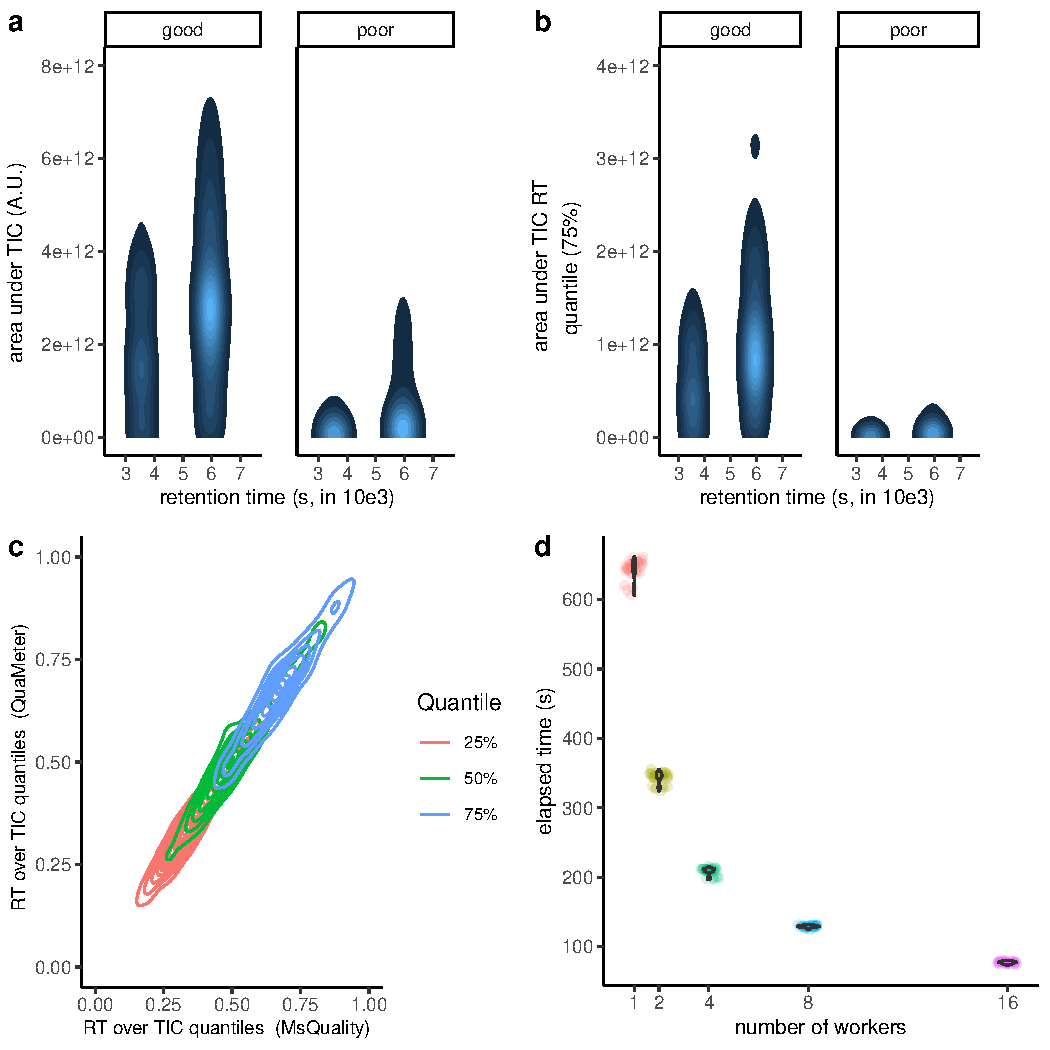
\includegraphics[scale=0.421]{figure-main}
 	  \caption{Examples of \texttt{MsQuality} functionality. Metrics are based
 	        on MS1 spectra; one data point is obtained per MS1 spectra\fixme{spectrum?}.
 	        (a) Area under TIC: The area under the total ion chromatogram. \fixme{$x$-axis is ugly (10e3)}
            (b) Quantiles of area under the total ion
                chromatogram of the retention time (TIC RT), here, the 75\% quantile. 
            (c) Comparison of quality metrics calculated by \texttt{MsQuality} 
                and QuaMeter: RT over TIC quantiles. \fixme{please show the actual points, not just a density!! see also \url{https://www.huber.embl.de/msmb/03-chap.html\#sec-graphics-2d} - hexbin \url{https://www.huber.embl.de/msmb/03-chap.html\#fig-graphics-twodsp6-2}}
            For (a), (b), and (c), the data points are displayed 
                as 2D densities and stratified for high-quality and low-quality
                measurements as classified in \cite{Amidan2014} or by the
                quantiles 25\%, 50\%, and 75\%. Brighter areas correspond to 
                high 2D density areas.
            (d) Wall-clock execution time for the calculation of quality metrics of the 
                data set of \cite{Amidan2014} when parallel computing is used 
                (1, 2, 4, 8, and 16 workers). A.U. arbitrary units.
    } \label{fig:fig1}
\end{figure}

The versatility of \texttt{MsQuality} in calculating metrics extends to a wide range of
applications, from small-scale studies to long-term acquisition of mass spectrometry
data. \fixme{define what you mean by long-term acquisition? a core facility running an
  instrument for months and years?}  We demonstrate the utility of \texttt{MsQuality} in
two case studies: a dataset of 180 cancer cell lines obtained by flow injection analysis
\citep{Cherkaoui2022} and a liquid chromatography (LC)-MS dataset of the same \emph{control sample}
\citep{Amidan2014} as instance of a long-term quality control usage scenario.  The values computed by \texttt{MsQuality}
agree with those of other data quality tools \fixme{plural appropriate here? you only show Quameter}, such as \fixme{why 'such as'? Be specific, precise, and laconic.} QuaMeter \citep{Ma2012}
(Fig. \ref{fig:fig1} c) or MatrixQCvis \citep{Naake2022}\fixme{ where is the comparison with MatrixQCvis shown?} \fixme{As it is written, it sounds like MsQuality just duplicates Quameter and therefore is not very novel? what is the point of having it?}. Correlating the
\texttt{MsQuality} metrics to the pre-calculated QuaMeter metrics by \citet{Amidan2014} showed
that 75\% of the analyzed metrics showed Pearson correlation coefficients over 0.81 and
Spearman correlation coefficients over 0.87 (see the Supplementary Data for further
details). \fixme{this sentence is awkaward (repetition of 'showed' and 'correlating/correlation')--entr\"umpeln}

\texttt{MsQuality} is implemented as an open-source\fixme{Pls specify the license, open-source is rather vague} R package, building upon the
established \texttt{Spectra} and \texttt{MsExperiment} packages
\citep{Rainer2022} to provide and represent the MS data. Thus, \texttt{MsQuality} supports a large variety of data input formats
as well as analyses of very large experiments through the use of data
representations with low memory footprint. Native parallelization enables a fast
and scalable calculation of quality metrics (Fig. \ref{fig:fig1} d, 
see the Supplementary Data for further details).

Finally, \texttt{MsQuality} requires little programmatic interaction and is designed to be
user-friendly.  After the instantiation of \texttt{Spectra} or \texttt{MsExperiment}
objects \fixme{why plural?}, a single function call is needed to calculate the quality metrics.


\section{Conclusion}

The software tool, \texttt{MsQuality}, contributes to the expanding list of 
tools that use the \texttt{Spectra}/\texttt{MsExperiment} framework to address 
various stages in the analysis pipeline of mass spectrometry data.
The implementation of \texttt{MsQuality}'s metric calculation is designed
to be user-friendly and streamlined and requires little programmatic 
interaction, facilitating reproducible calculation and evaluation of data 
quality metrics.

By building upon an extensive ecosystem for mass spectrometry data, centered
around the \texttt{Spectra} and \texttt{MsExperiment} packages \citep{Rainer2022},  \fixme{third repetition of the same point in as many paragraph. Please trim.}
\texttt{MsQuality} enables researchers to create seamless analysis workflows 
for rapid, efficient, and standardized evaluation of MS data quality, 
ultimately leading to more robust scientific discoveries in mass spectrometry
workflows.


\section{Acknowledgements}

We acknowledge feedback from the SMART-CARE consortium \fixme{few people will know who or what that is. Better to list the actual names, even if many} on usability of 
\texttt{MsQuality} and all developers and maintainers of the R/Bioconductor 
packages \texttt{MsQuality} is built upon. We would like to thank Nicola Zamboni
for his valuable assistance in locating and understanding the data of Cherkaoui et al. (2022). \fixme{why not use $\backslash$citet here?}

\subsection{Author contributions statement}

T.N. conceptualized the project. T.N. and J.R. implemented the algorithms as an R
package. T.N. analysed the results. W.H. provided feedback and guidance. T.N., J.R. and
W.H. wrote the manuscript.

\subsection{Funding}

This work was supported by the Bundesministerium für Bildung und Forschung 
[grant agreement no. 161L0212E].

Conflict of Interest: none declared.




\begin{thebibliography}{}

\bibitem[Amidan \textit{et~al}., 2014]{Amidan2014}
Amidan, B.G. \textit{et~al} (2014) Signatures for mass spectrometry data
quality.
\textit{Proteome Research}, \textbf{13}, 2215--2222.

% \bibitem[Bereman, 2015]{Bereman2015}
% Bereman, M.S. (2015) Tools for Monitoring System Suitability in LC MS/MS 
% Centric Proteomic Experiments.
% \textit{Proteomics}, \textbf{15}, 891--902.

\bibitem[Bittremieux \textit{et~al}., 2017]{Bittremieux2017}
Bittremieux, W. \textit{et~al} (2017) Computational quality control tools for
mass spectrometry proteomics.
\textit{Proteomics}, \textbf{17}, 1--11.

\bibitem[Cherkaoui \textit{et~al}., 2022]{Cherkaoui2022}
Cherkaoui, S. \textit{et~al} (2022) A functional analysis of 180 cancer cell
lines reveals conserved intrinsic metabolic programs.
\textit{Molecular Systems Biology}, \textbf{18}, e11033.

\bibitem[K\"ocher \textit{et~al}., 2011]{Koecher2011}
K\"ocher, T. \textit{et~al} (2011) Quality control in LC-MS/MS.
\textit{Proteomics and Systems Biology}, \textbf{11}, 1026--1030.

% \bibitem[Paulovich \textit{et~al}., 2010]{Paulovich2010}
% Paulovich, A.G. \textit{et~al} (2010) Interlaboratory Study Characterizing a 
% Yeast Performance Standard for Benchmarking LC-MS Platform Performance.
% \textit{Molecular \& Cellular Proteomics}, \textbf{9}, 242--254.

\bibitem[Ma \textit{et~al}., 2012]{Ma2012}
Ma, Z.-Q. \textit{et~al} (2012) QuaMeter: Multivendor Performance Metrics
for LC–MS/MS Proteomics Instrumentation.
\textit{Analytical Chemistry}, \textbf{84}, 5845--5850.

\bibitem[Naake \textit{et~al}., 2022]{Naake2022}
Naake, T. \textit{et~al} (2022) MatrixQCvis: shiny-based interactive data
quality exploration for omics data.
\textit{Bioinformatics}, \textbf{38}, 1181--1182.

\bibitem[Rainer \textit{et~al}., 2022]{Rainer2022}
Rainer, J. \textit{et~al} (2022) A Modular and Expandable Ecosystem for Metabolomics Data Annotation in R.
\textit{Metabolites}, \textbf{12}, 173.

\end{thebibliography}


%\bibliographystyle{natbib}
%\bibliographystyle{achemnat}
%\bibliographystyle{plainnat}
%\bibliographystyle{abbrv}
%\bibliographystyle{bioinformatics}

%\bibliographystyle{plain}

\bibliography{../supplement/document.bib}

\end{document}
 
